% Charlotte Geiger - Manuel Lippert - Leonard Schatt
% Physikalisches Praktikum

% Teilaufgabe 6

\section{Kreiselkompass}
Bei einem rotierender Kreisel auf dem keine Drehmomente wirken, behält der Drehimpuls seine Richtung bei, weswegen ein Kreisel als Kompass geeignet ist, wobei einKreiselkompass auf den geographischen Nordpol zeigt. Für eine kräftefreien Kreisel wird eine sogenannte \enquote{Cardano-Aufhängung} verwendet, welche verhindert, dass die Schwerkraft auf den Kreisel ein Drehmoment auswirken kann, was eine Drehimpulsänderung zur Folge hätte. In der Cardano Aufhängung wird dann der Kreisel möglichst reibungsfrei auf zwei sich im Schwerpunkt des Kreisels senkrecht schneidenden Achsen gelagert. Ein Kreiselkompass wird auch zur Navigation im Weltraum verwendet, was heutzutage schon in Satelliten und Sonden umgesetzt wird. \footnote{Bergmann-Schäfer, Lehrbuch der Experimentalphysik Band 1, S.278}
\begin{center}
    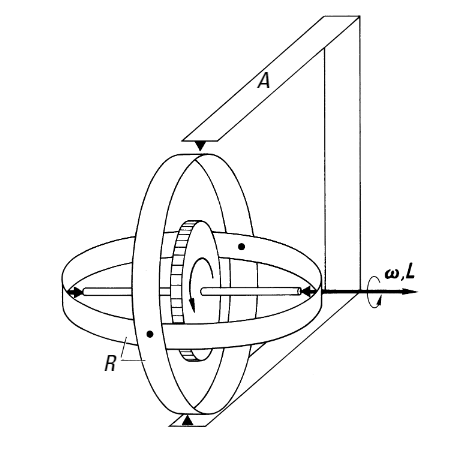
\includegraphics[width = 5.5cm]{KraeftefreieAufhaengung.PNG}
    \captionof{figure}{Kräftefreie Aufhängung eines Kreisels / Cardano-Aufhängung}
\end{center}